\section{Homepage}

L'homepage di un sito web rappresenta l'equivalente di una vetrina per un 
negozio. L'obiettivo della homepage è quello di introdurre l'utente e di 
presentare le informazioni essenziali nel modo più efficace possibile. 
Infatti, l'homepage deve tener conto dell'identità del soggetto che 
rappresenta (in questo caso l'azienda), della navigazione, della velocità 
di presentazione dei contenuti e di strumenti (ad esempio, la ricerca). 

\subsection{6W}

Ai fini della valutazione di come l'informazione viene presentata, si 
analizzerà seguendo i 6 assi: \textit{Where}, \textit{Who}, \textit{Why}, 
\textit{What}, \textit{When}, \textit{How}. 

\subsubsection{Where}

\centerline{\textit{A quale sito sono arrivato? Che tipo di contenuto mi 
propone il sito web?}}
È possibile notare a primo impatto uno slogan che permette di intuire 
direttamente il tema di cui l'azienda tratta (fig. \ref{fig:homepage-1}). 
Inoltre, è possibile vedere a primo impatto anche che l'azienda sviluppa 
un prodotto che può essere usufruito tramite dispositivi mobili. È 
possibile notare anche la frase posta sotto allo slogna, in cui viene 
spiegato qual è il prodotto che l'azienda sviluppa. 

\begin{figure}[H]
	\centering
	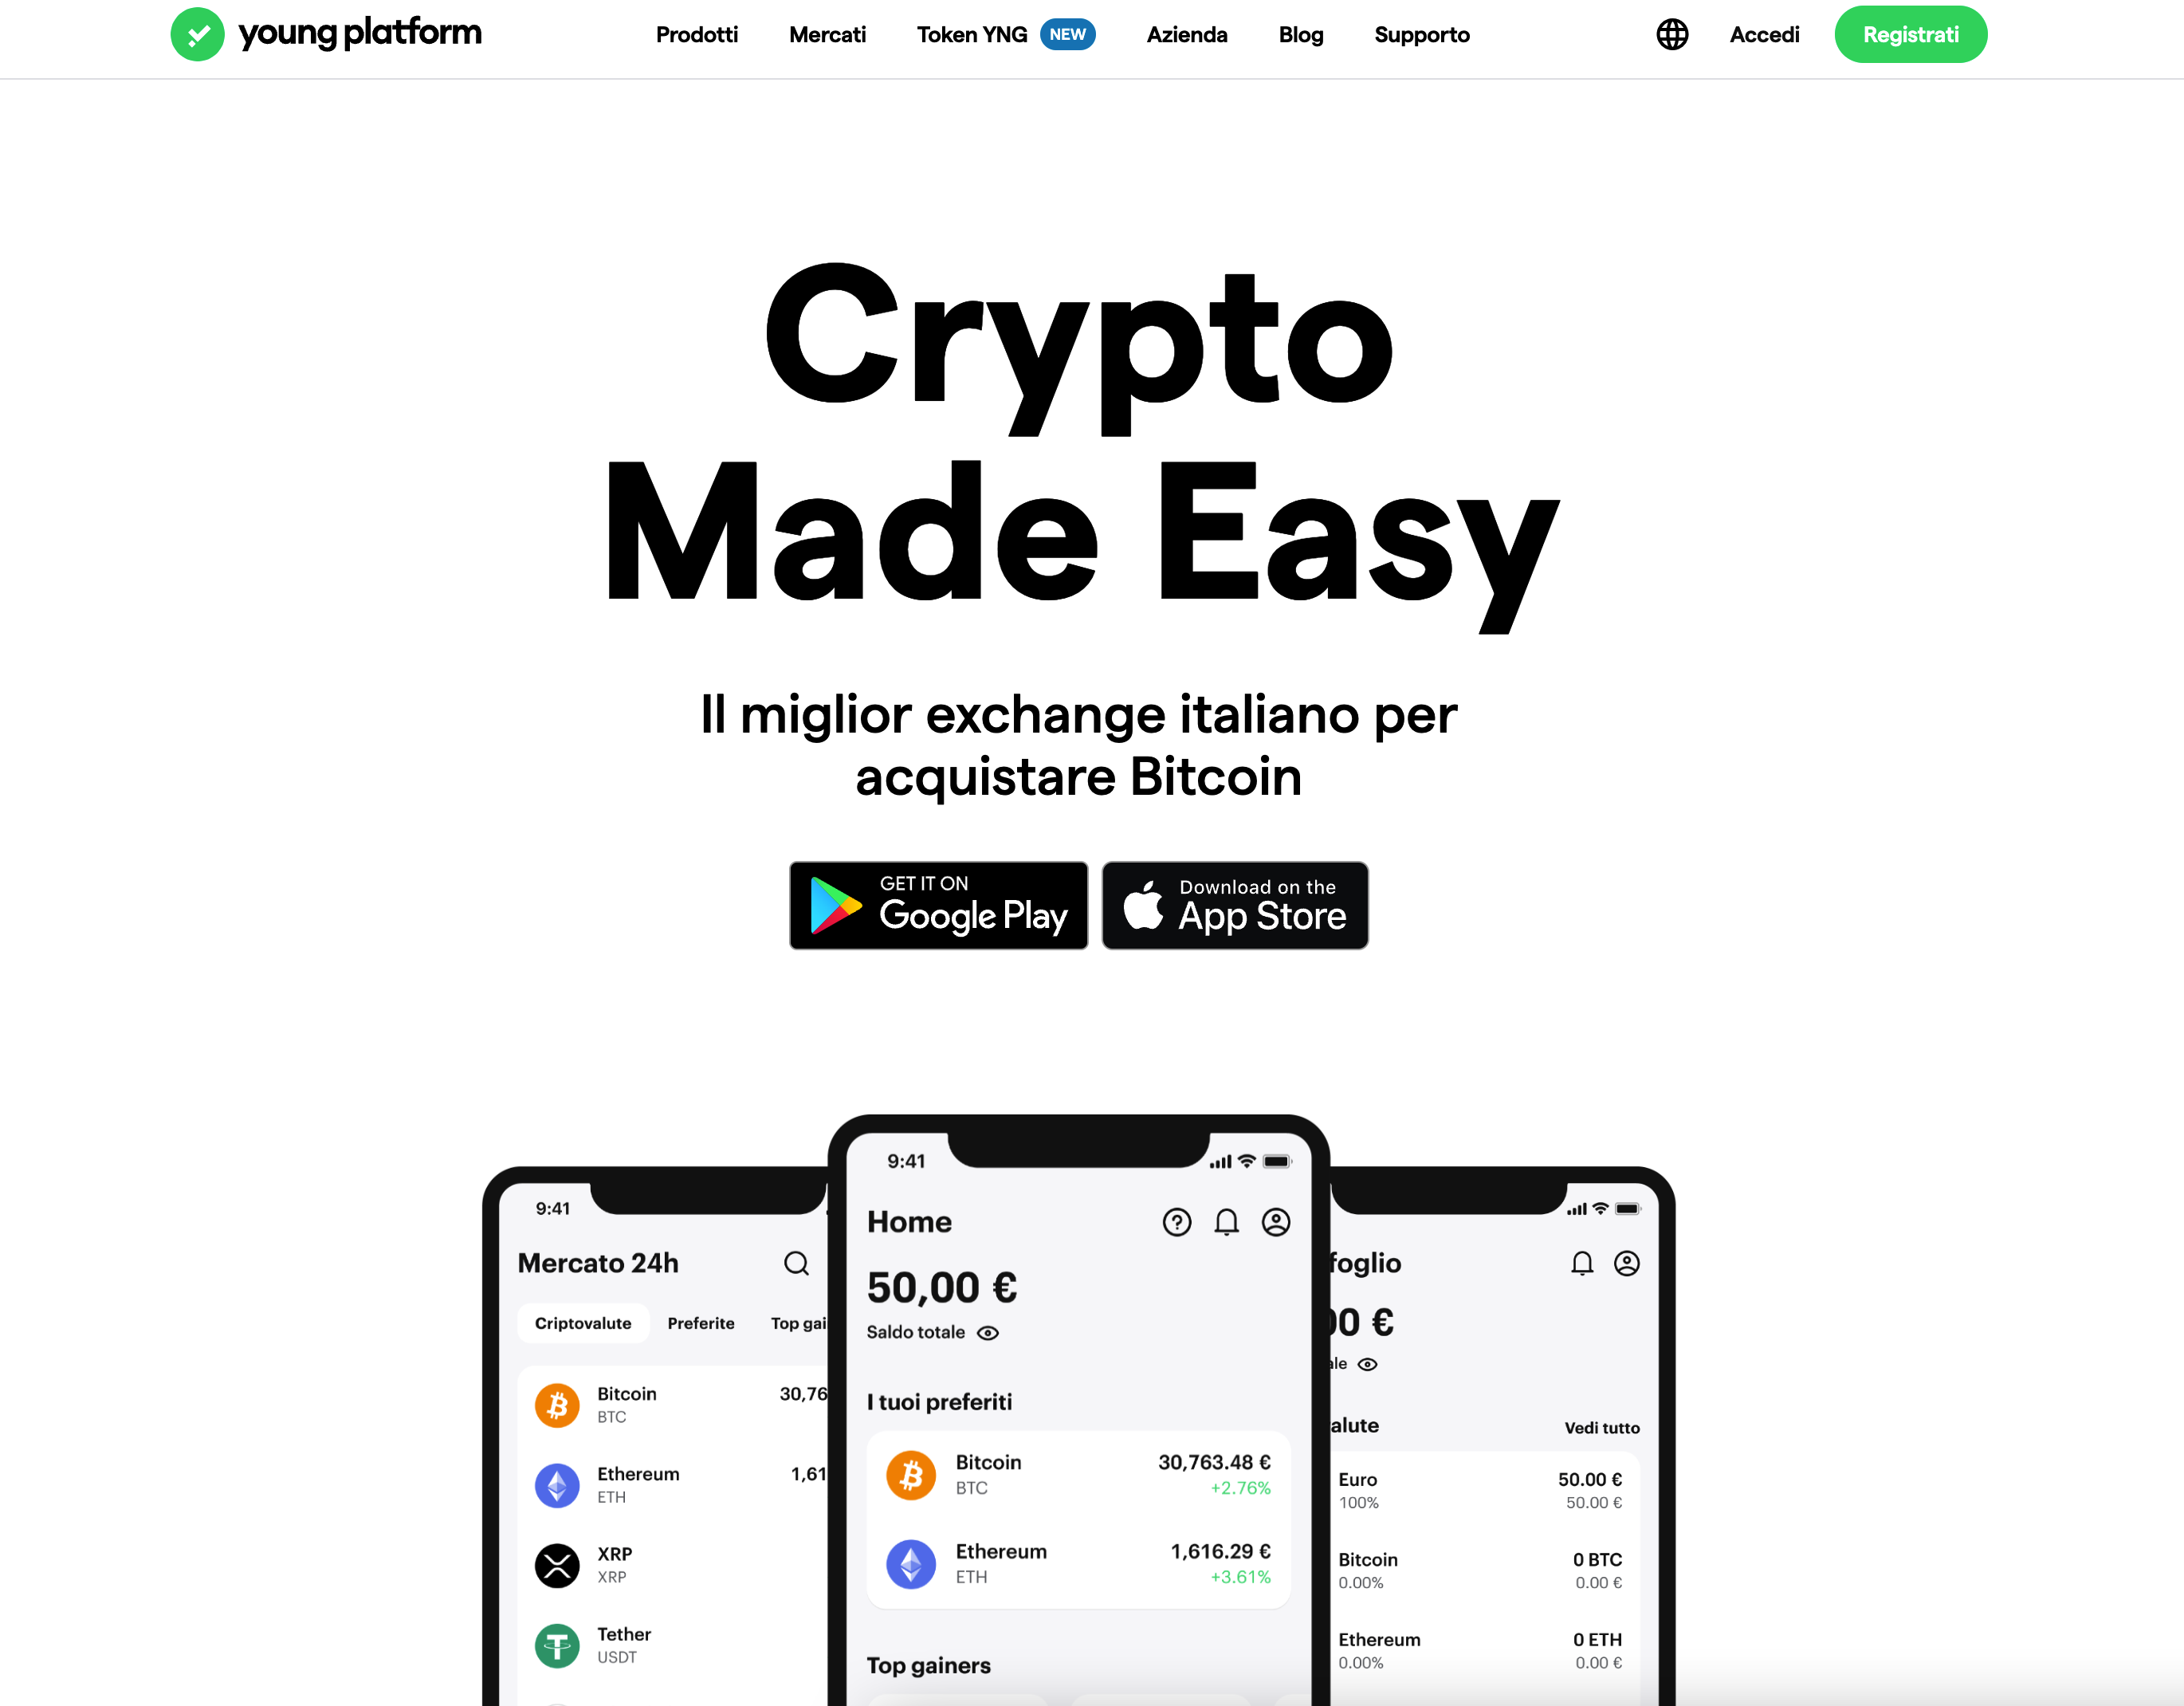
\includegraphics[width=0.80\textwidth]{res/images/homepage-1.png}
	\caption{Prima sezione della homepage.}
	\label{fig:homepage-1}
\end{figure}

\subsubsection{Who}

\centerline{\textit{Chi c'è dietro questo sito?}}
A primo impatto non è possibile capire chi c'è dietro a questo sito. Come 
detto in precedenza, il nome del sito web non permette di trarre alcuna 
informazione per poter intuire chi potrebbe essere dietro alla realizzazione 
del sito. Nel menù posto in alto al centro, è possibile notare la voce 
\textit{Azienda} e da lì si apre a sua volta un menù in cui è presente la 
voce \textit{Parlano di noi} (fig. \ref{fig:who-we-are-1}). Cliccando su tale 
voce, si viene reindirizzati in una pagina che raccoglie una serie di 
articoli che parlano dell'azienda (fig. \ref{fig:who-we-are-2}). Quindi, a 
prima vista non è facile capire qual è il team dietro al sito e di 
conseguenza chi ha realizzato questi prodotti. Per avere delle informazioni 
aggiuntive riguardo all'azienda è necessario quindi effettuare una ricerca 
preliminare. Questo dal punto di vista dell'utente questo rappresenta un 
grande svantaggio e potrebbe essere un motivo per non continuare con la 
visualizzazione del sito web. 

\begin{figure}[H]
	\centering
	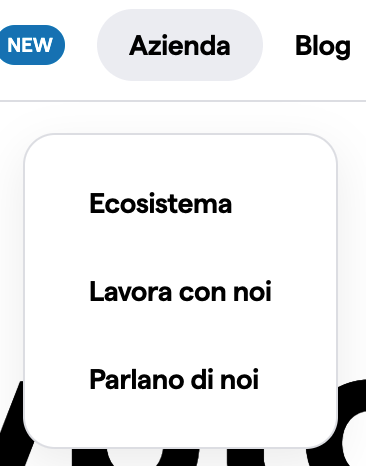
\includegraphics[width=0.30\textwidth]{res/images/who-we-are-1.png}
	\caption{Menù principale - Parlano di noi}
	\label{fig:who-we-are-1}
\end{figure}

\begin{figure}[H]
	\centering
	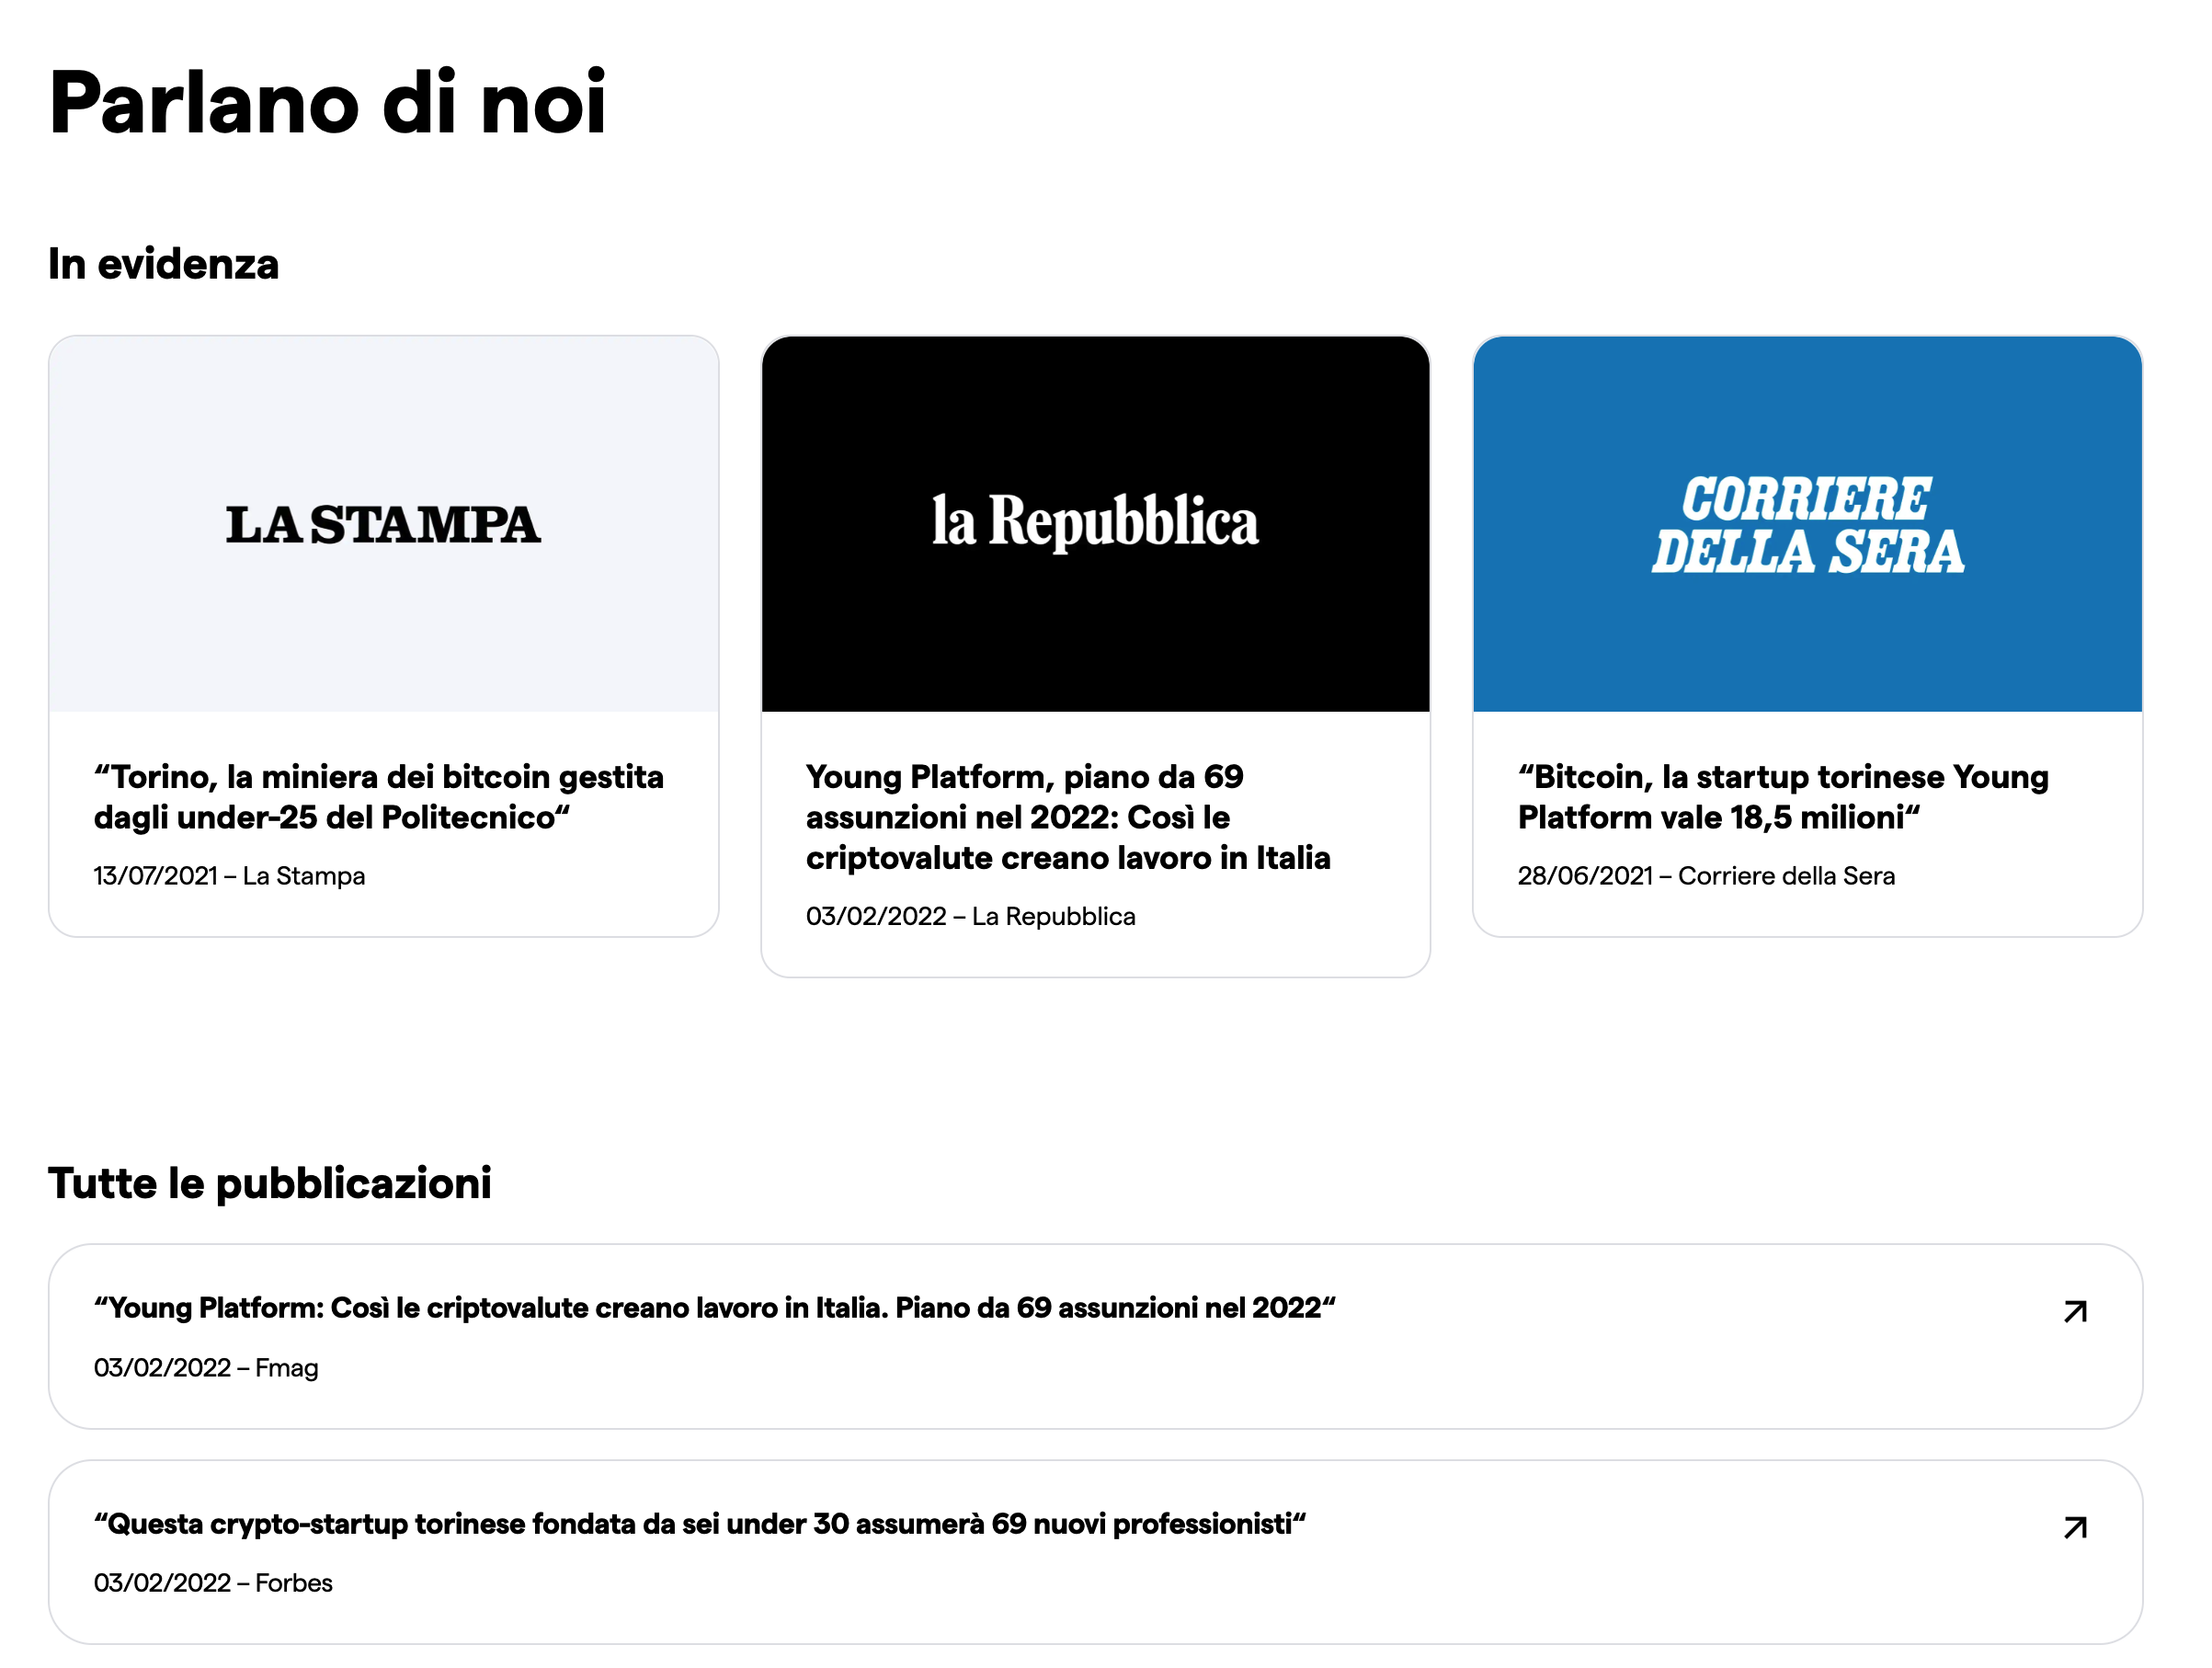
\includegraphics[width=0.80\textwidth]{res/images/who-we-are-2.png}
	\caption{Page \textit{Parlano di noi}}
	\label{fig:who-we-are-2}
\end{figure}

\subsubsection{Why}

\centerline{\textit{Perchè l'utente dovrebbe rimanere 
nel sito? Quali vantaggi offre?}}
L'obiettivo del sito è quello di attrarre principalmente l'attenzione di 
quegli utenti nuovi e che vogliono addentrarsi in questo mondo. Quindi, 
dal punto di vista di un utente neofita, il sito è invogliato a rimanere 
nel sito, in quanto può apprendere molte informazioni: dalle basi 
tecnologiche su cui si poggia questo fino alle ultime notizie del mondo 
crypto. Per un utente invece più esperto del settore, questo sito potrebbe 
non essere attratto in quanto il sito presenta principalmente dei contenti 
e dei prodotti indirizzati ai principianti. L'azienda ha sviluppato anche 
un prodotto dedicato ad utenti esperti, ma nel sito non viene fatto cenno 
di tale prodotto se non nel footer, alla voce \textit{Young Platform Pro} 
(seconda voce della prima colonna a sinistra) (fig. \ref{fig:footer}). 
Tuttavia, è necessario ricordare che l'obiettivo che si è posto l'azienda 
è quello di introdurre a questo settore il maggior numero di utenti 
principianti. Quindi, suppongo che un utente senza esperienza, rimanga 
molto interessato dai contenuti della homepage e che può trarne diversi 
benefici.

\begin{figure}[H]
	\centering
	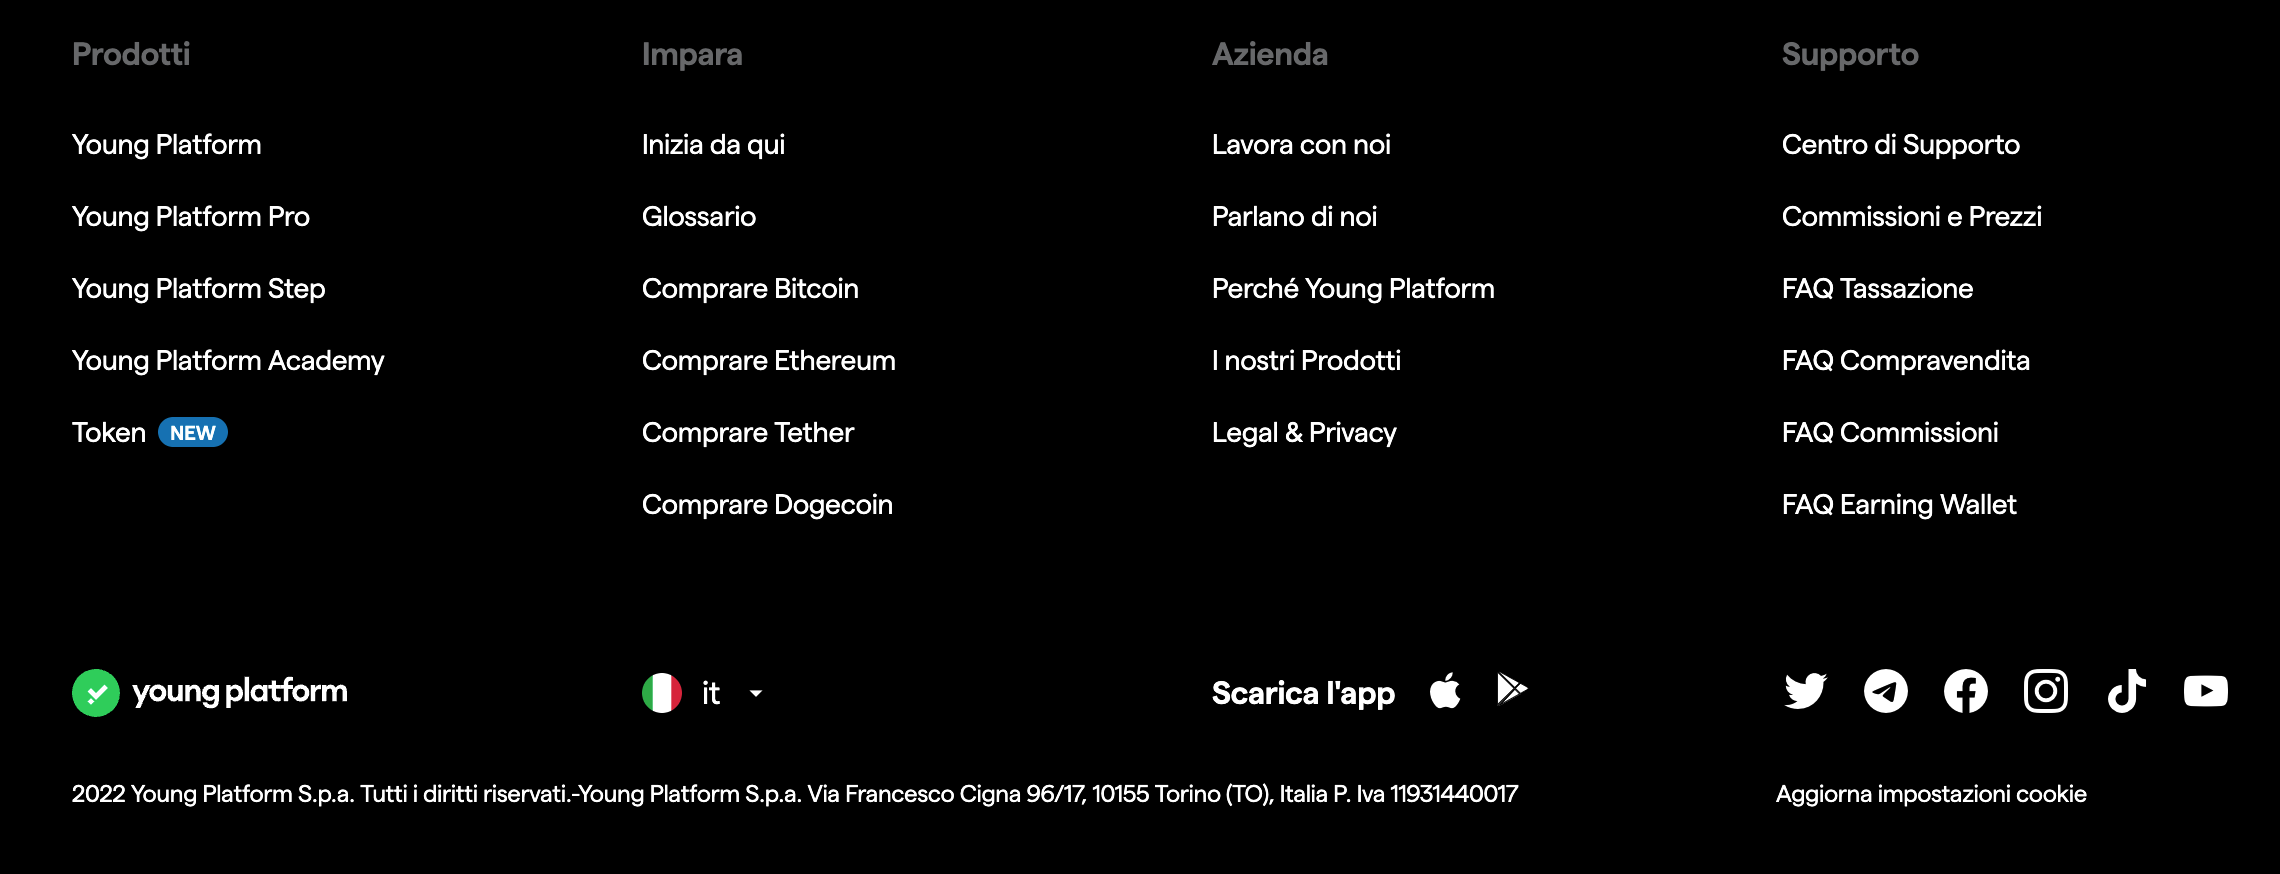
\includegraphics[width=0.80\textwidth]{res/images/footer.png}
	\caption{Footer del sito web.}
	\label{fig:footer}
\end{figure}

\subsubsection{What}

\centerline{\textit{Che cosa offre questo sito?}}
Questa homepage offre diverse sezioni che possono essere suddivise in:
\begin{itemize}
  \item \textit{Introduzione}: l'utente può vedere immediatamente uno 
  slogan, il settore su cui l'azienda si concentra e dei prodotti (delle 
  applicazioni per dispositivi mobili) (fig. \ref{fig:homepage-1});

  \item \textit{Introduzione al mondo delle criptovalute}: questa sezione, 
  posta poco dopo la sopra citata, ha lo scopo di introdurre gli utenti 
  neofiti a questo mondo. L'azienda ha collaborato con un importante 
  personaggio televisivo degli anni duemila legato ad un programma televisivo 
  per bambini. L'aver messo il volto di tale persona permette ad un neofita 
  di rassicurarsi e che può essere guidato da una persona che è in grado 
  di utilizzare uno stile comunicativo semplice e chiaro. Ritengo che 
  questa sezione sia molto importante per invogliare gli utenti a continuare 
  a visitare il sito (fig. \ref{fig:introduction-1});
  \begin{figure}[H]
    \centering
    
\includegraphics[width=0.80\textwidth]{res/images/introduction-1.png}
    \caption{Sezione che introduce dei contenuti per utenti neofiti.}
    \label{fig:introduction-1}
  \end{figure}

  \item \textit{Processo dalla registrazione all'utlizzo del prodotto}: 
  si illustra brevemente quali sono i passaggi principali per poter 
  utilizzare il prodotto dell'azienda e per entrare nel mondo delle 
  criptovalute (fig. \ref{fig:registration-process});
  \begin{figure}[H]
    \centering
    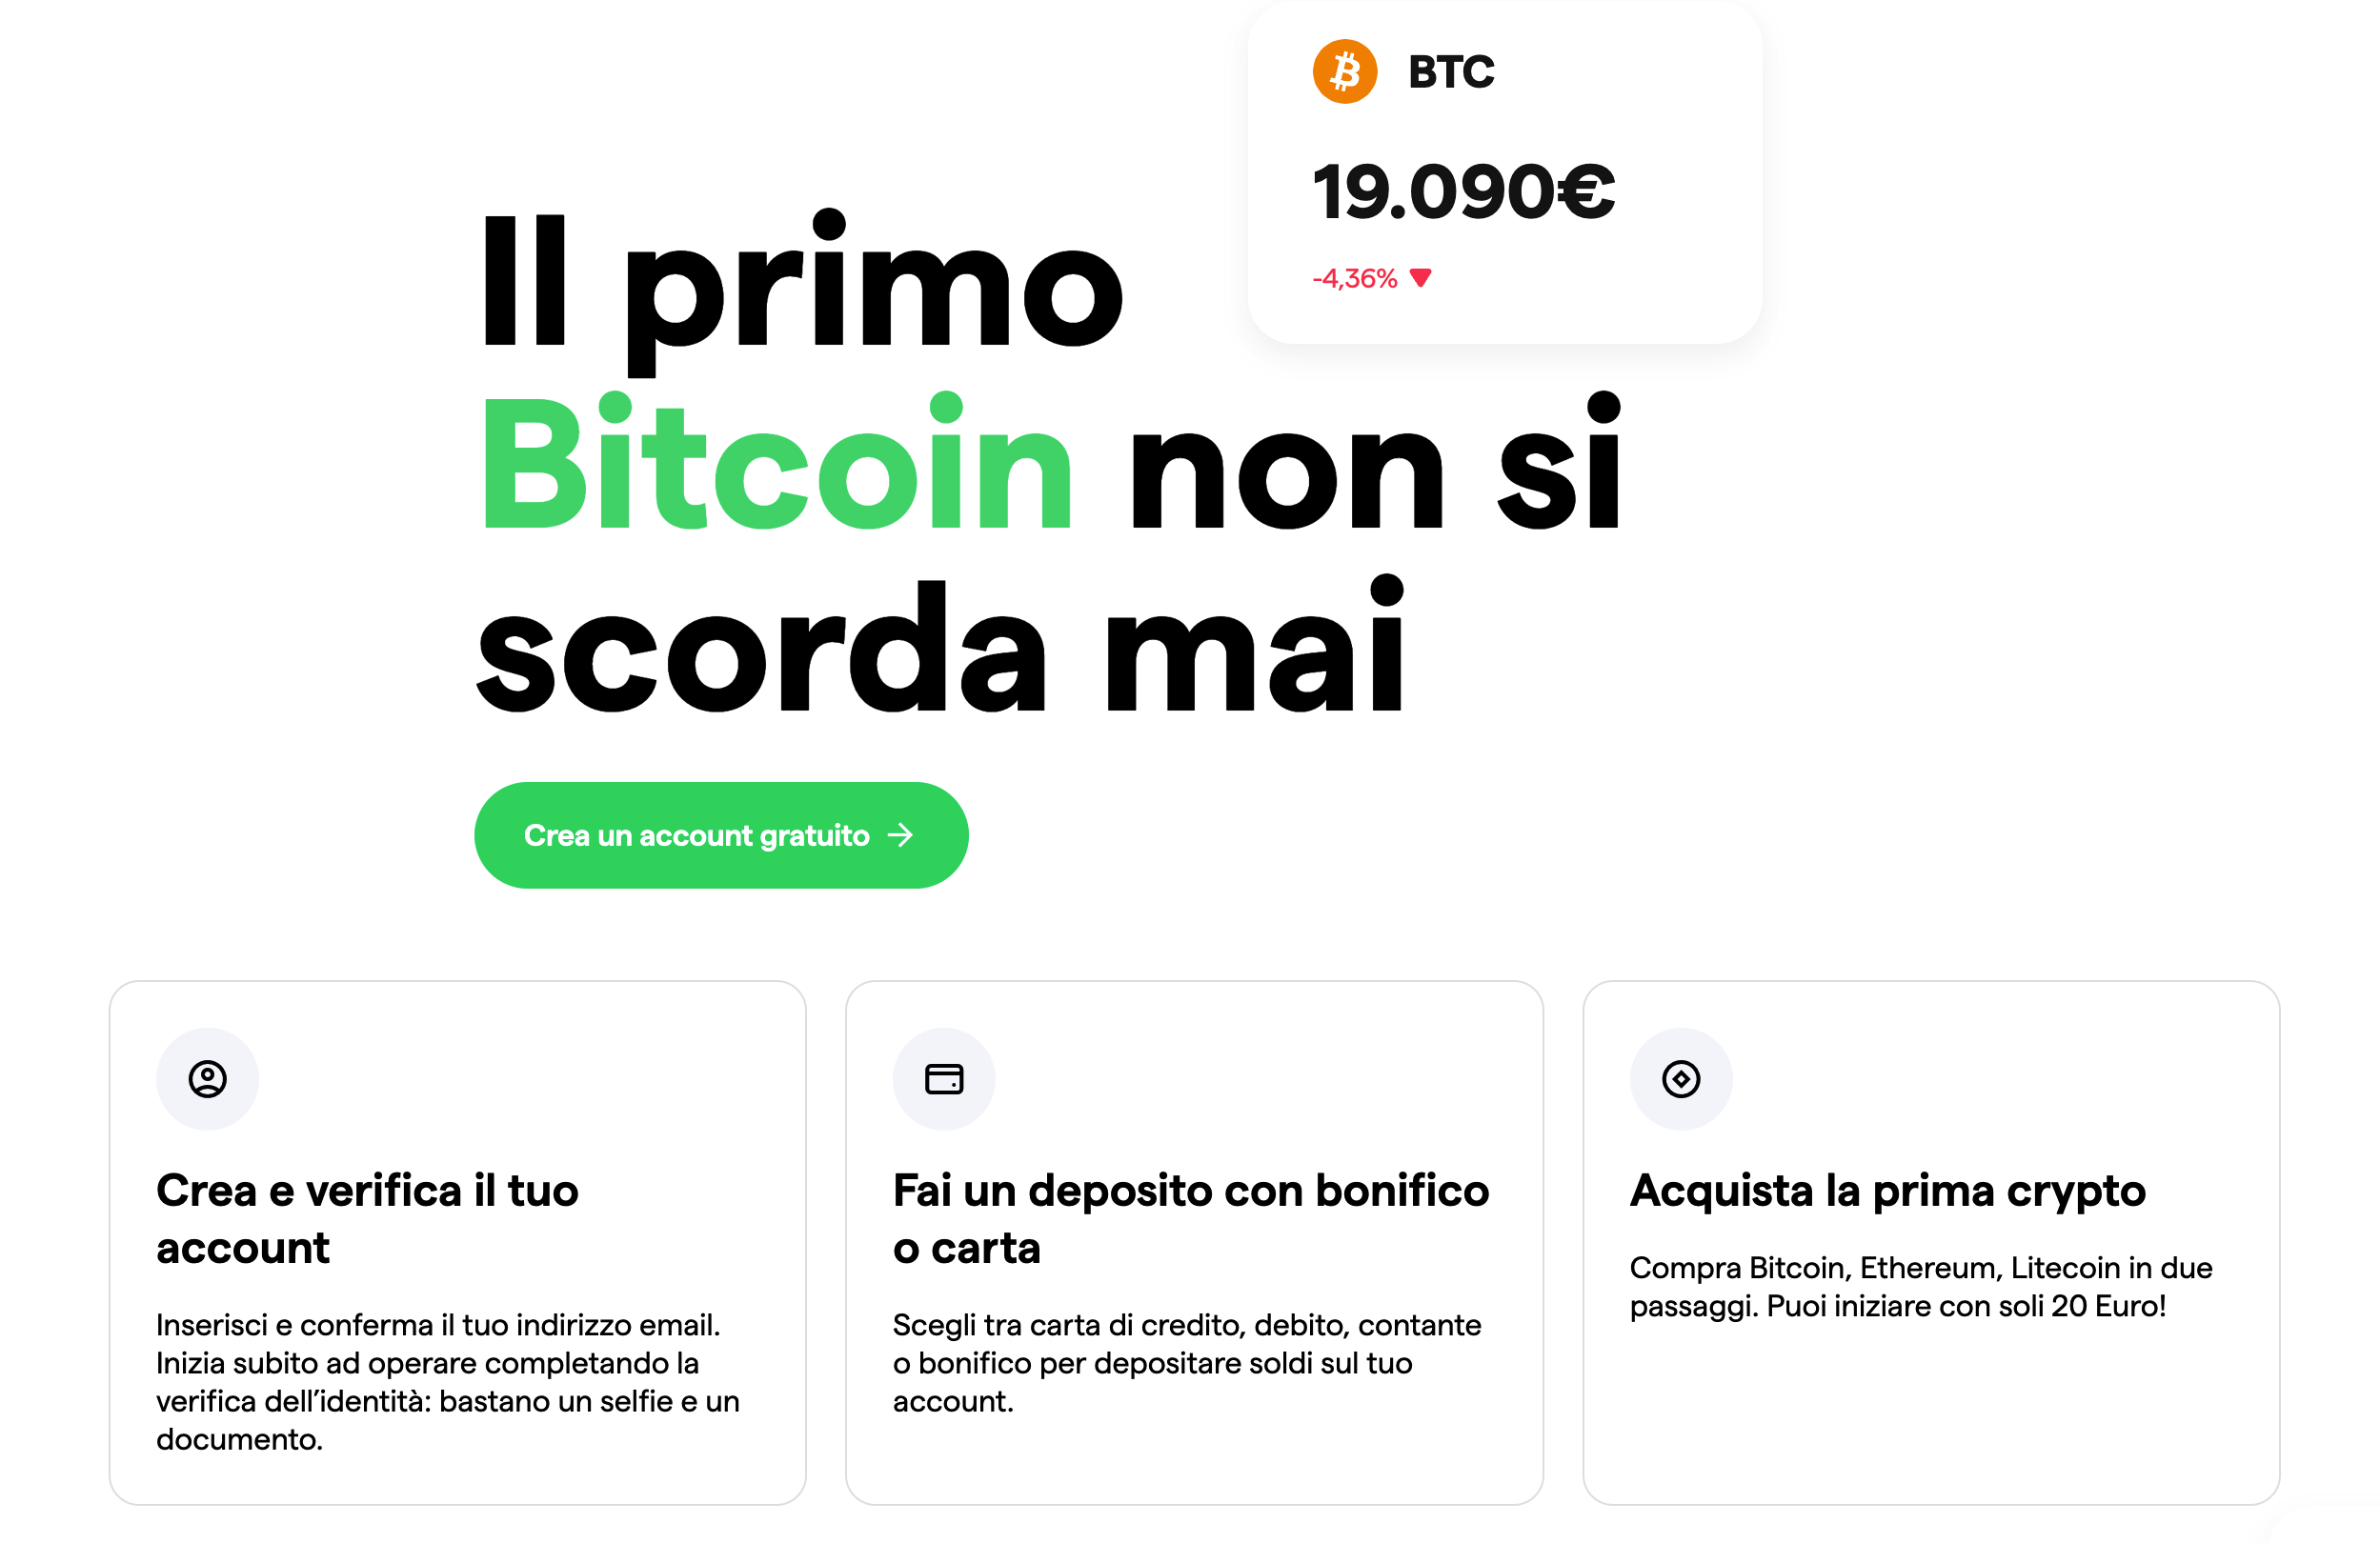
\includegraphics[width=0.80\textwidth]{res/images/registration-process.png}
    \caption{Passi principali per l'utilizzo del prodotto offerto dall'azienda.}
    \label{fig:registration-process}
  \end{figure}

  \item \textit{Informazioni sui depositi}: essendo le criptovalute un 
  campo che richiede da parte dell'utente un investimento di una certa 
  somma di denaro, il sito illustra una sezione che rassicura l'utente 
  che è possibile utilizzare diverse modalità per depositare dei fondi 
  nell'applicazione (fig. \ref{fig:deposit-options});
  \begin{figure}[H]
    \centering
    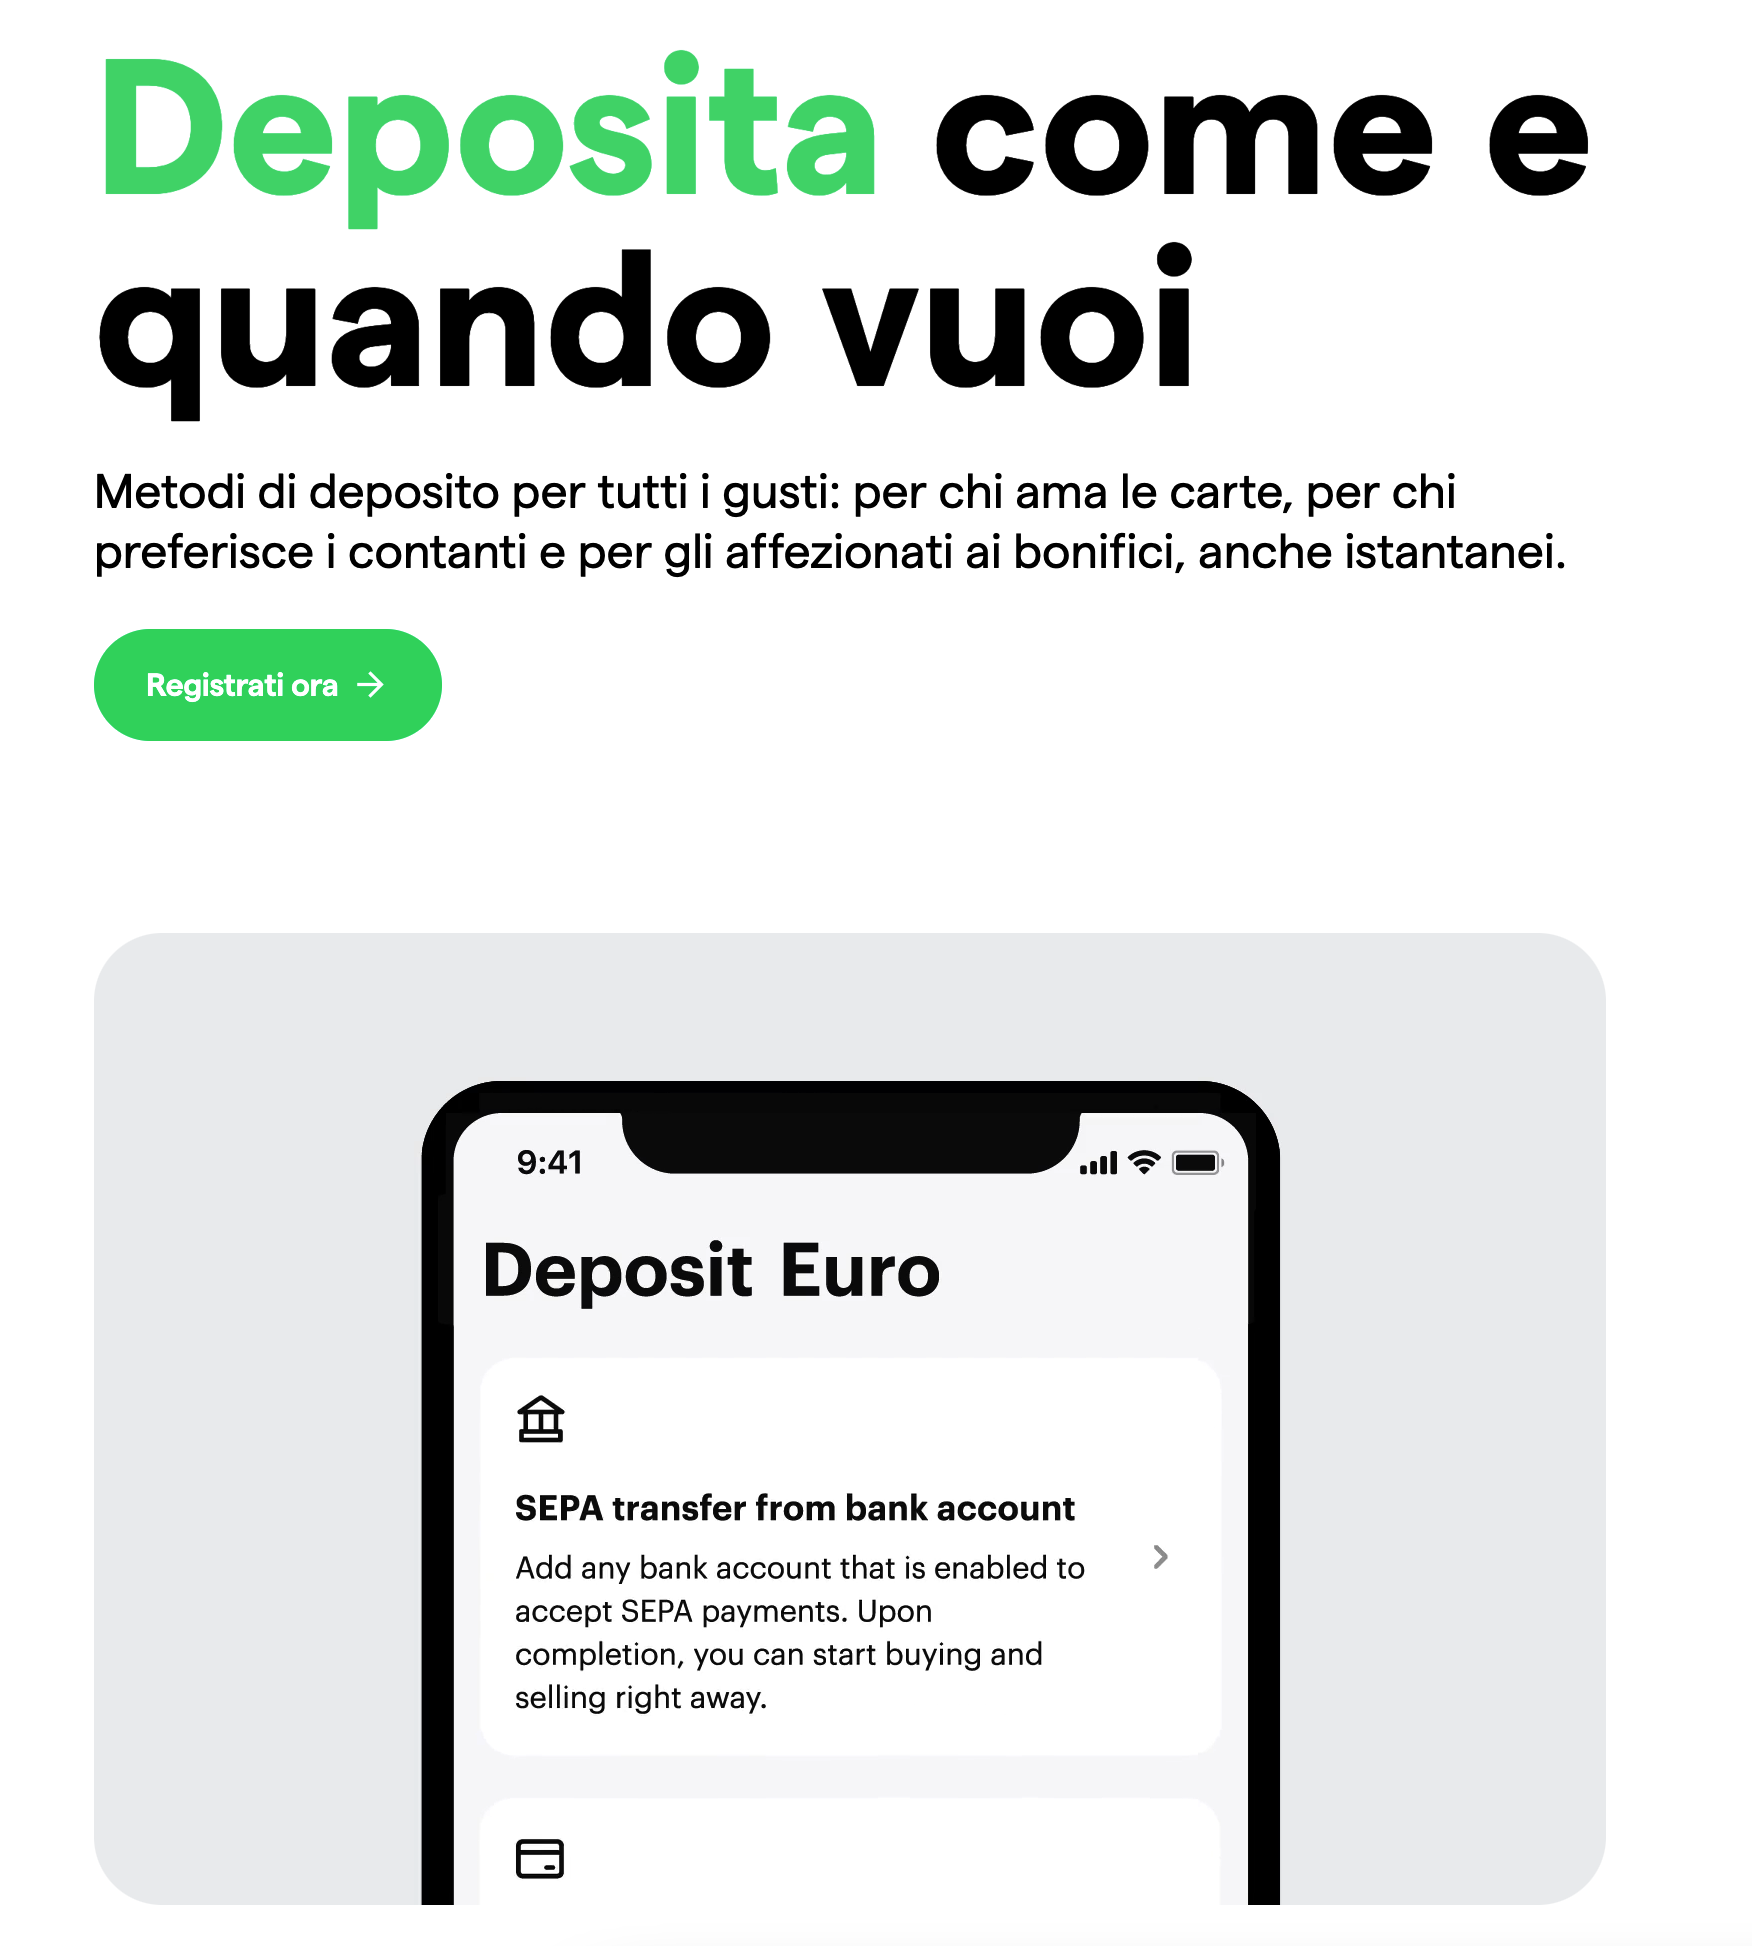
\includegraphics[width=0.50\textwidth]{res/images/deposit-options.png}
    \caption{Informazioni sulle tipologie di depositi offerti dal prodotto.}
    \label{fig:deposit-options}
  \end{figure}

  \item \textit{Academy, articoli per l'apprendimento}: questa è un'altra 
  sezione dedicata agli utenti neofiti con lo scopo di rassicurarli. Infatti, 
  l'obiettivo è quello che l'utente verrà guidato passo passo, partendo 
  dalle fondamenta tecnologiche della blockchain, fino ai concetti più 
  avanzati delle criptovalute (fig. \ref{fig:academy}).
  \begin{figure}[H]
    \centering
    
\includegraphics[width=0.60\textwidth]{res/images/academy.png}
    \caption{Sezione che introduce gli articoli per l'apprendimento 
    delle fondamenta del settore crypto.}
    \label{fig:academy}
  \end{figure}
\end{itemize}

\subsubsection{When}

\centerline{\textit{Il sito web è aggiornato?}}
Quando si raggiunge il sito per la prima volta non è possibile capire se 
il sito è aggiornato. Tuttavia, un modo per verificare ciò è quello di 
accedere alla pagina \textit{Blog}, facilmente raggiungibile dal menù 
centrale in alto. Da tale pagina è possibile notare che vengono pubblicati 
settimanalmente diversi articoli che riguardano le ultime situazioni del 
mercato delle criptovalute e le novità introdotte nei prodotti offerti 
dall'azienda. Per ogni articolo, viene indicata la data di pubblicazione 
(fig. \ref{fig:blog}). Inoltre, viene indicata anche una stima del tempo 
di lettura dell'articolo, in modo che l'utente può avere una prima idea se 
può al momento leggere un determinato articolo piuttosto che un altro.

\begin{figure}[H]
	\centering
	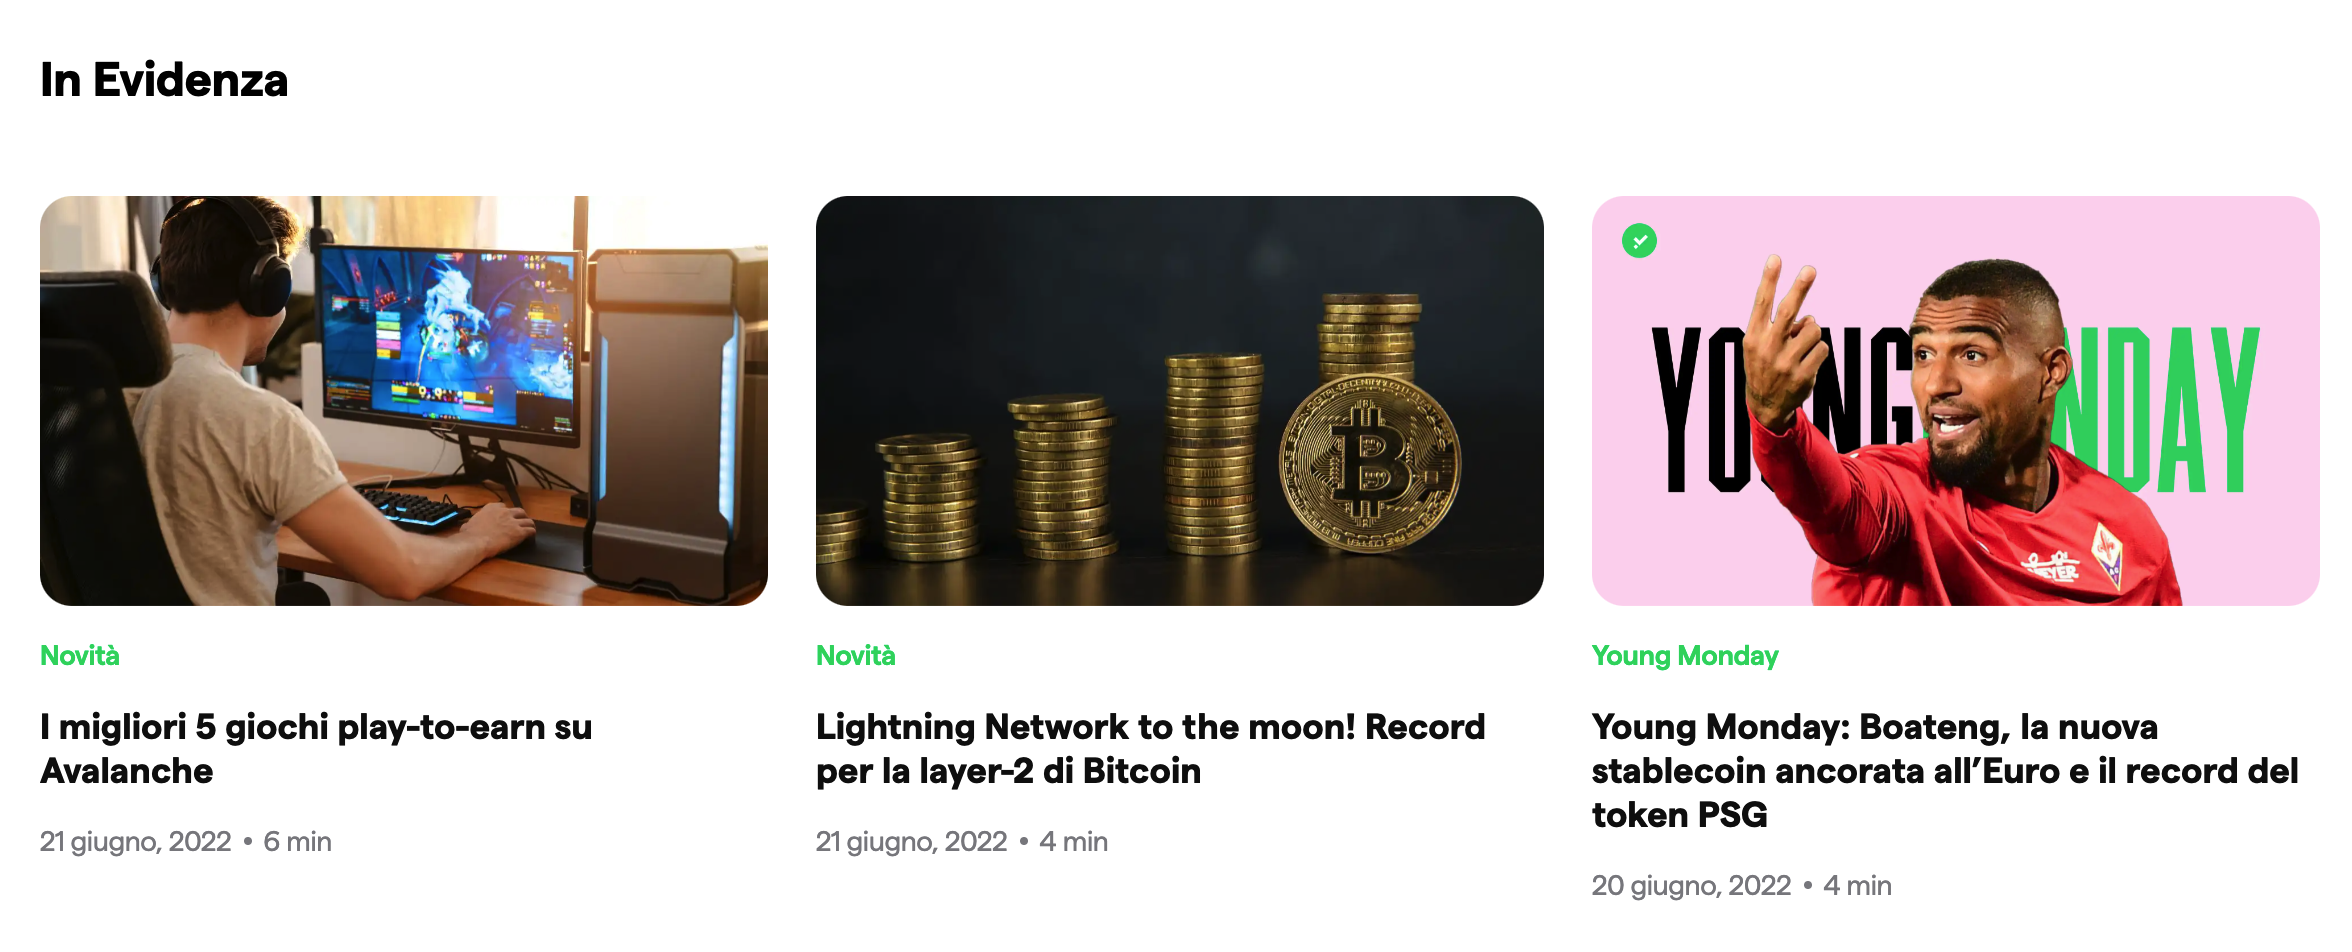
\includegraphics[width=0.90\textwidth]{res/images/blog-1.png}
	\caption{Alcuni articoli del blog.}
	\label{fig:blog}
\end{figure}

\subsubsection{How}

\centerline{\textit{Come può l'utente raggiungere quello che gli 
interessa?}}
Nella homepage è possibile raggiungere con una certa semplicità:
\begin{itemize}
  \item dove potersi registrare a accedere per usufruire dei prodotti;
  \item accedere ai contenuti per l'apprendimento del mondo della 
  blockchain e delle criptovalute;
  \item il blog, una sezione per poter rimanere aggiornato sulle ultime 
  notizie strettamente collegate al mondo crypto;
  \item le FAQ;
  \item il supporto, che per questa tipologia di prodotti è molto 
  importante, sopratutto per utenti neofiti. Nonostante l'obiettivo 
  dell'azienda sia quello di rendere il fruibile e accessibile l'utilizzo 
  delle criptovalute, il supporto rappresenta un punto di riferimento molto 
  importante per l'utente: le criptovalute introducono delle nuove 
  conoscenze e delle nuove dinamiche con cui l'utente deve col tempo avere 
  dimistichezza. Il sito, per evidenziare l'importanza di questa sezione, 
  ha posto la rispettiva voce nel menù principale, in modo che l'utente 
  possa raggiungerla molto facilmente e si trova in una posizione facile 
  da ricordare (fig. \ref{fig:main-menu}).

  \begin{figure}[H]
    \centering
    
\includegraphics[width=0.90\textwidth]{res/images/main-menu.png}
    \caption{Menù principale della homepage.}
    \label{fig:main-menu}
  \end{figure}
\end{itemize}

Analizzando il menù principale è possibile notare che è stato posto in un 
posto ben visibile. Di seguito si illustrino le voci:
\begin{itemize}
  \item \textit{Prodotti}: quando il cursore passa sopra a questa voce, 
  compare un sottomenù. Ogni voce di questo sottomenù presenta uno dei 
  prodotti offerti dall'azienda e ogni voce reindirizza ad una specifica 
  pagina;

  \item \textit{Mercati}: questa voce reindirizza ad una pagina che 
  illustra l'andamento del mercato delle criptovalute;
  
  \item \textit{Token YNG}: questa voce reindirizza ad una pagina che 
  introduce il token creato dall'azienda;

  \item \textit{Azienda}: quando il cursore passa sopra a questa voce, 
  compare un sottomenù. Ogni voce di questo sottomenù reindirizza ad una 
  specifica pagina. Le voci di questo sottomenù sono:
  \begin{itemize}
    \item \textit{Ecosistema}: reindirizza ad una pagina in cui viene 
    illustrato tutto l'ecosistema dei prodotti sviluppati dall'azienda;
    \item \textit{Lavora con noi}: reindirizza ad una pagina in cui 
    l'azienda illustra i valori in cui credono e una lista di offerte 
    lavorative;
    \item \textit{Parlano di noi}: reindirizza ad una pagina il cui 
    contenuto è parzialmente illustrato nella figura \ref{fig:who-we-are-2};
  \end{itemize}

  \item \textit{Blog}: reindirizza ad una pagina in cui sono raccolti 
  tutti gli articoli che riguardano le ultime notizie del mercato dell 
  criptovalute;

  \item \textit{Supporto}: reindirizza ad una pagina nella quale l'utente 
  può contattare il supporto dell'azienda per necessità.
\end{itemize}

Il fatto che alcune voci non reindirizzano ad una pagina ma mostrano un 
sottomenù a tendina rende il sito poco prevedibile dal punto di vista 
dell'utente. Tuttavia, questa tipologia di sottomenù sono facile da 
navigare. Il sottomenù della voce \textit{Azienda} si esapande 
verticalmente, che è preferibile rispetto ad una espansione orizzontale. 
Il sottomenù della voce \textit{Prodotti} invece si esapande in maniera 
differente: il contenuto del sottomenù è una griglia di due righe e due 
colonne. Ogni voce contiene il nome del prodotto, una versione del logo 
aziendale con un colore differente per ogni prodotto e una breve 
descrizione del prodotto. Vengono suddivisi i prodotto in due categorie: 
i prodotti per \textit{appassionati di criptovalute} e 
\textit{principianti in criptovalute} (fig. \ref{fig:products-submenu}). 
Così facendo, si è realizzato un sottomenù ricco di informazioni e che 
guida l'utente verso la scelta del prodotto adatto all'utente. Ritengo che 
sarebbe stato più utile scambiare di posizione le due colonne, in modo da 
dare più importanza ai prodotti dedicati ai principianti. Il fatto di 
aver utilizzato un colore differente del logo aziendale per ogni prodotto 
è molto utile per l'utente, in quanto può riconoscere più facilmente un 
prodotto rispetto all'altro. Un svantaggio di questi sottomenù è che non 
sono \textit{fault tolerant}, ovvero, non appena il cursore non punta sulla 
voce con il sottomenù, questi scompaiono.
\begin{figure}[H]
  \centering
  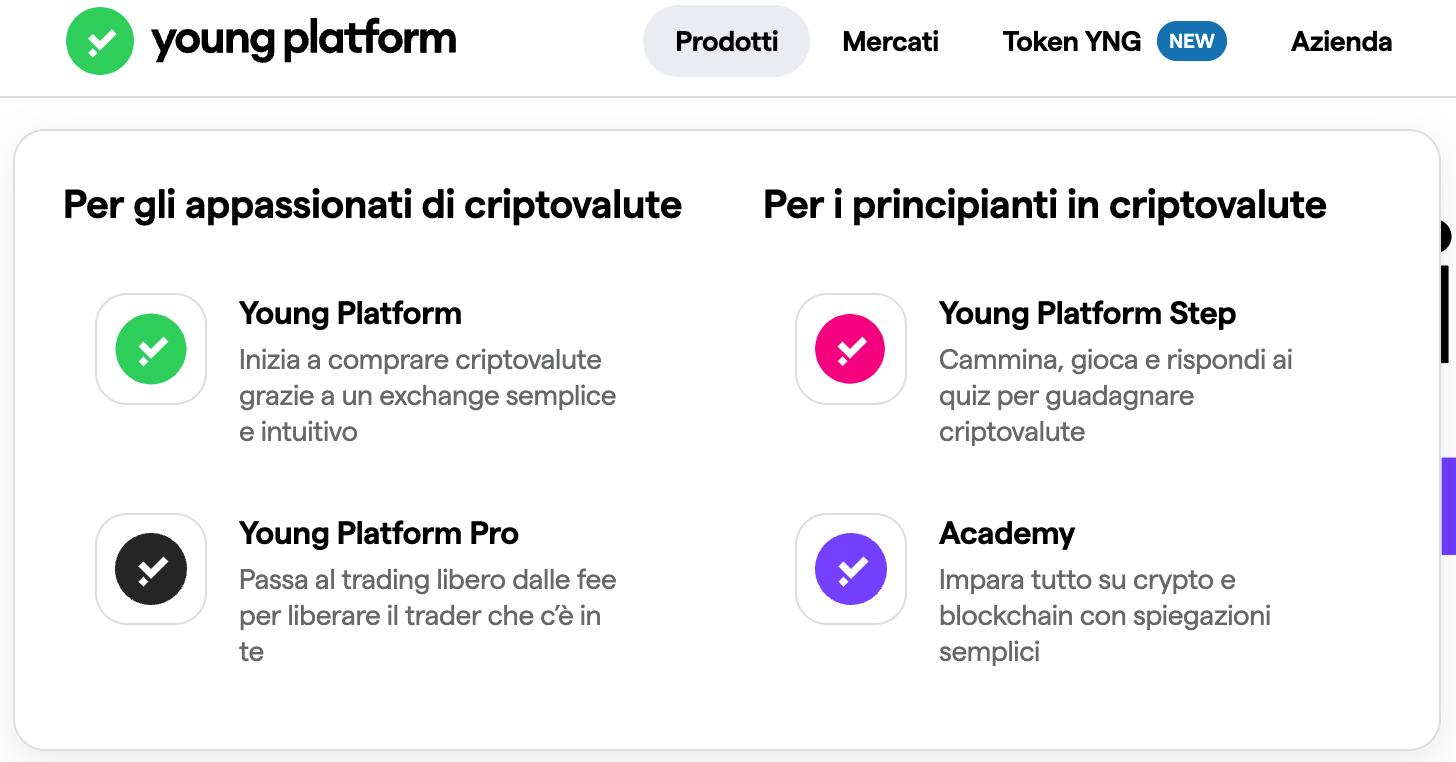
\includegraphics[width=0.70\textwidth]{res/images/products-submenu.png}
  \caption{Sottomenù della voce \textit{Prodotti}.}
  \label{fig:products-submenu}
\end{figure}